\documentclass[10pt,aspectratio=169]{beamer}

\usepackage[english]{babel}
\usepackage{t1enc}
\usepackage{pgfpages}
\usepackage{array}

\usetheme{default}
\setbeamercovered{transparent}
\setbeamertemplate{navigation symbols}{}
\setbeamertemplate{footline}{
\usebeamercolor[fg]{title}%
\hfill\insertframenumber{}/\inserttotalframenumber \phantom{xx}
}

\usepackage{enumitem}
\setlist[itemize]{label=\textcolor{blue}{$\bullet$}}


\newcommand{\blue}{\color{blue}}
\newcommand{\red}{\color{red}}
\newcommand{\black}{\color{black}}
\newcommand{\darkred}{\color{darkred}}
\newcommand{\darkgreen}{\color{darkgreen}}

\begin{document}
\title{Using \texttt{mk}\\
  Linking against shared libraries}
\author{Alberto Artoni}
\date{01/03/2024}

\begin{frame}
  \maketitle
\end{frame}

\section{Toolchains, \texttt{mk}, libraries and header files}

\begin{frame}{Toolchains}
    A \textbf{toolchain} is a set of software which constitutes a close environment for the development of further software.
    The toolchain encapsulates:
  \begin{itemize}
      \item a compiler (and related standard library)
  \item a linker
  \item basic tools for software development
  \item basic libraries for scientific development
  \end{itemize}	

    The software \textbf{must} be independent from the hosting OS.

\end{frame}

\begin{frame}{How do I confine my work inside a specific toolchain?}

    The \texttt{Bash} environmental variables define paths for executables and libraries; the tool to manage these variables is commonly called the \textbf{environment module system}.

  There are two main module systems, the one we use is named \texttt{Lmod} (the other is \texttt{TCL Environment Modules}).\\[3mm]

    A \textbf{module} is basically a set of instructions that define a specific environment for a specific software: where are the \textit{executables}, where are its \textit{libraries}, where are the \textit{header files}, $\dots$

    \underline{If the software is built inside a toolchain, the installation and the environment  will be portable.} \\[3mm]

A specific module is “loaded” and can be “unloaded” as well when not needed.
The module system can define a hierarchy: a module may need another one, and the system automatically handles these dependencies.

\end{frame}

\begin{frame}[fragile]

  Initialization of \texttt{mk}

\begin{verbatim}
$ source /u/sw/etc/bash.bashrc

$ module avail
---------- /u/sw/modules/toolchains ----------
gcc-glibc/11.2.0 (D)
\end{verbatim}

Choice of the toolchain
\begin{verbatim}
$ module load gcc-glibc/11.2.0
\end{verbatim}

Inside the toolchain I can find a lot of packages
\begin{verbatim}
$ module avail
\end{verbatim}
\end{frame}


\begin{frame}[fragile]
  \small
  Now a specific software package can be selected: usually many other requested modules will be automatically loaded
\begin{verbatim}
$ module avail
---------- /u/sw/pkgs/toolchains/gcc-glibc/11.2.0/modules ----------
R/4.1.0                gsl/2.7         (L)    pybind11/2.6.2
adol-c/2.7.2    (L)    hdf5/1.12.0     (L)    qhull/2020.2       (L)
arpack/3.8.0    (L)    hypre/2.22.0    (L)    qrupdate/1.1.2     (L)
blacs/1.1       (L)    lis/2.0.30             scalapack/2.1.0    (L)
boost/1.76.0    (L)    matio/1.5.21    (L)    scipy/1.7.0        (L)
cgal/5.3               metis/5.1.0     (L)    scotch/6.1.1       (L)
dakota/6.15.0          mumps/5.4.0     (L)    suitesparse/5.10.1 (L)
dealii/9.3.1    (L)    netcdf/4.8.0    (L)    superlu/5.3.0      (L)
eigen/3.3.9     (L)    octave/6.2.0    (L)    tbb/2021.3.0       (L)
fenics/2019.1.0        openblas/0.3.15 (L)    trilinos/13.0.1    (L)
fftw/3.3.9      (L)    p4est/2.3.2     (L)    vtk/9.0.3          (L)
glpk/5.0        (L)    petsc/3.15.1    (L)
\end{verbatim}

The module system takes care of the integrity of the definitions and does not permit bad cross-coupling (e.g. libraries with an incompatible \texttt{libc}).\smallskip

To unload all the loaded modules:
\begin{verbatim}
$ module purge
\end{verbatim}
\end{frame}


\begin{frame}[fragile]

  The module system takes care of defining the environment variable \texttt{LD\_LIBRARY\_PATH} so the loader can find newly loaded libraries.

  The user is responsible of passing compiler and linker flags when compiling, to do so they must know where libraries and headers are located.

  The module system provides variables to make it easy to find headers and libraries of loaded modules

\begin{verbatim}
$ module load eigen
$ module list
Currently Loaded Modules:
1) gcc-glibc/11.2.0   2) eigen/3.3.9

$ echo ${mkEigenInc}
/u/sw/pkgs/.../eigen/3.3.9/include/eigen3
\end{verbatim}
\end{frame}

\begin{frame}{Naming scheme for in our toolchain}
General naming scheme: 
\begin{itemize}
\item Installation path: \texttt{"mk" + Modulename + "Prefix"}, \textit{e.g.} \texttt{\$\{mkOctavePrefix\}}
\item Headers: \texttt{"mk" + Modulename + "Inc"}, \textit{e.g.} \texttt{\$\{mkEigenInc\}}
\item Libraries: \texttt{"mk" + Modulename + "Lib"}, \textit{e.g.} \texttt{\$\{mkSuitesparseLib\}}
\end{itemize}

\end{frame}

\begin{frame}[fragile]{How to use a third-party library}
  Basic compile/link flags:
\begin{verbatim}
$ g++ -I${mkLibrarynameInc} -c main.cpp
$ g++ -L${mkLibrarynameLib} -llibraryname main.o -o main
\end{verbatim}
\bigskip
\textbf{Warning}: by mistake, one can include headers and link against libraries related to different installations/versions of the same library! The compile, link and loading phase may succeed, but the executable may crash, resulting in a very subtle yet painful error to debug!
\end{frame}

\section{Some useful things to remember about shared libraries}

\begin{frame}{Using shared libraries}
   Shared libraries:
   \begin{itemize}
       \item User point of view
       \item Developer point of view
   \end{itemize}

  \medskip
   Users need to take care to 
   \begin{itemize}
       \item \textbf{linking} phase during compilation
       \item \textbf{loading} phase at execute time
   \end{itemize}

  \medskip
   Developers usually contribute to a
   \begin{itemize}
       \item \textbf{development} phase
       \item \textbf{release} phase
   \end{itemize}

\end{frame}


\begin{frame}{Versions and releases} 
  The \emph{version} is a symbol
  (typically a number) by which we indicate a set of instances of a
  library with a common public interface and functionality.
  \smallskip

    Within a version, one may have several \textit{releases}, typically indicated
  by one or more numbers (major and minor or bug-fix). A new release is 
  issue to fix bugs  or improve of a library without
  changes in its public interface. So a code linked against version 1,
  release 1 of a library should work (in principle) when you update
  the library to version 1, release 2.
  \smallskip

  Normally version and releases are separated by a dot in the library name:
  \texttt{libfftw3.so.3.3.9} is version 3, release 3.9 of the
  \texttt{fftw3} library (The Fastest Fourier Transform in the West).

  \begin{center}
      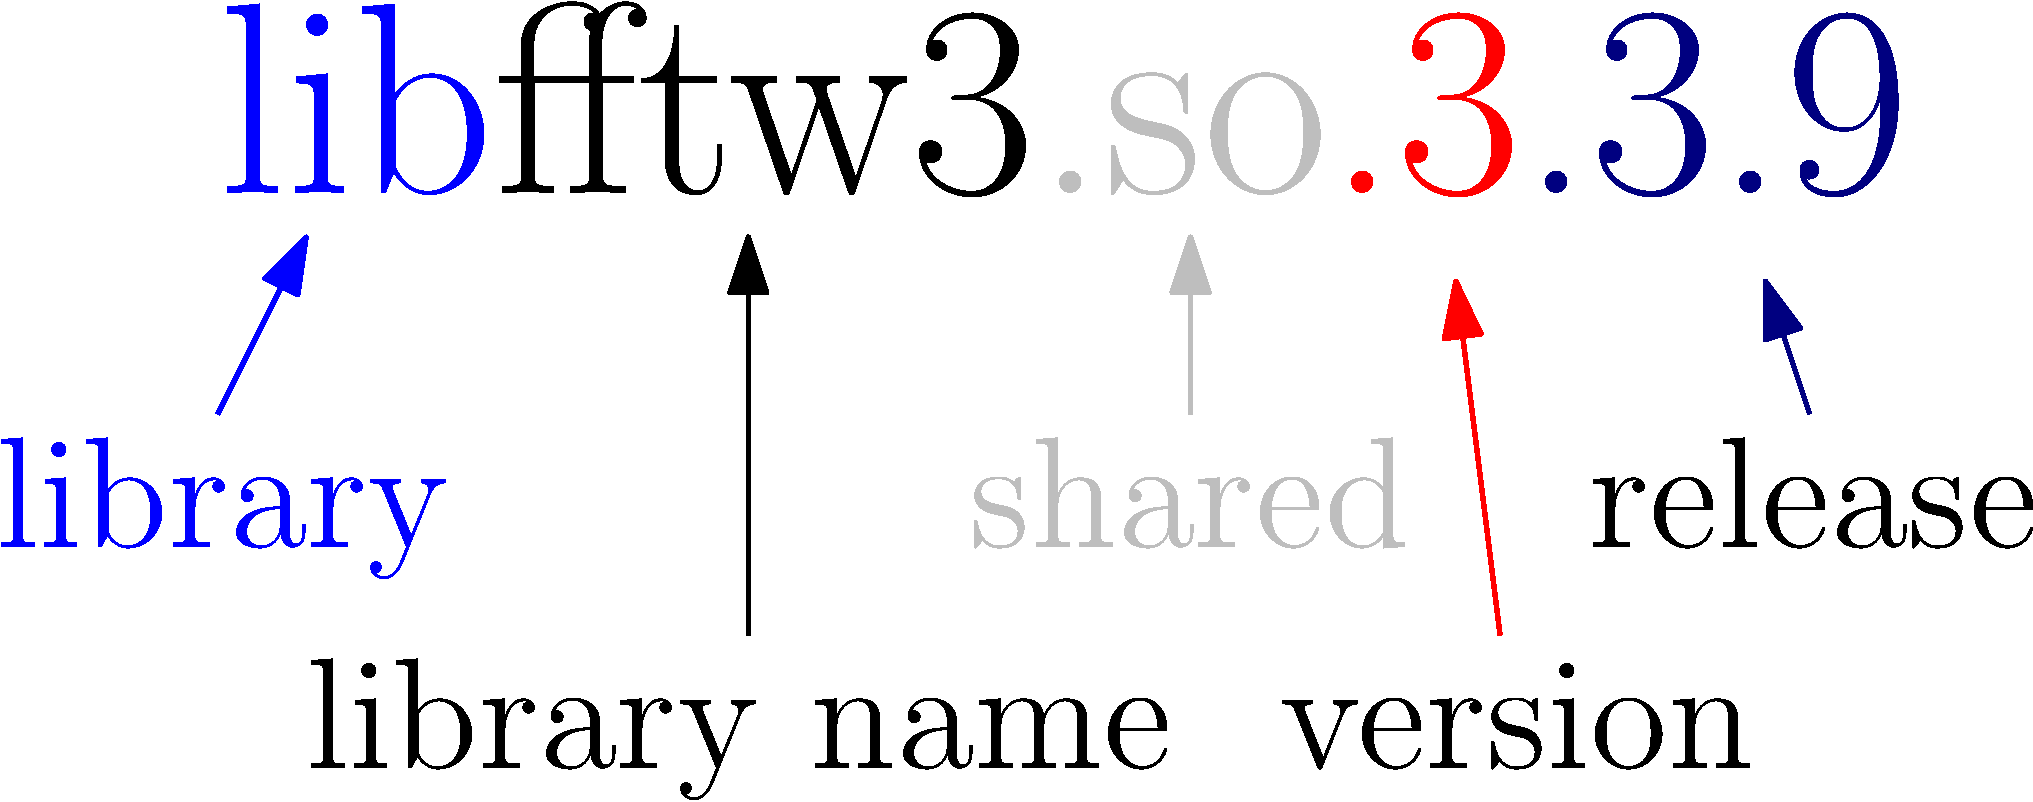
\includegraphics[width=0.45\textwidth]{ipe/libExplained.pdf}
  \end{center}

\end{frame}

\begin{frame}[fragile]{Naming scheme of shared libraries (Linux/Unix)}
  We give some nomenclature used when describing a shared library

  \begin{itemize}
      \item \textbf{link name}: name used in the linking stage when
    you use the \texttt{-lmylib} option.  
    \item \textbf{soname}: \textit{shared object name} looked after
    by the \emph{loader} stage.  
\item \textbf{full name}: name of the actual file that stores the library. 
  \end{itemize}
\medskip

    Example:
    \begin{itemize}
        \item[] \texttt{fftw}: is the \textit{link name}.
        \item[] \texttt{libfftw3.so.3}: is the \textit{soname}.
        \item[] \texttt{libfftw3.so.3.3.9}: is the \textit{real name} of the file.
    \end{itemize}

    We call a \textit{fully qualified library} a soname that contains the full path to the library.
\end{frame}


\begin{frame}[fragile]{How does it work?}  The command
  \texttt{ldd} lists the shared libraries used by an object file. \\
  \medskip
  
\textbf{Example:}
\begin{verbatim}
$ ldd ${mkOctavePrefix}/lib/octave/6.2.0/liboctave.so
...
libfftw3.so.3 =>
     /u/sw/toolchains/gcc-glibc/11.2.0/pkgs/fftw/3.3.9/lib/libfftw3.so.3
...
\end{verbatim}
\begin{itemize}
	\item \texttt{Octave} has been linked to \texttt{libfftw3}.
\end{itemize}

The \textbf{loader} searches the occurrence of this library, finding his full qualified name. \\ \medskip

\textbf{Which release?} 
\begin{verbatim}
$ ls -l ${mkFftwLib}/libfftw3.so.3
/full/path/to/libfftw3.so.3 -> libfftw3.so.3.3.9
\end{verbatim}
I am in fact using release \texttt{3.9} of version \texttt{3}.
\end{frame}

\begin{frame}{Got it?}  

  The executable (\texttt{octave}) contains the
  information on which shared library to load, including version
  information (its \texttt{soname}). This part has been taken care by the 
  developers of \texttt{Octave}.
  \smallskip

  When I launch the program the loader looks in special directories,
  among which \texttt{/usr/lib} for a file that matches the
  \texttt{soname}. This file is typically a symbolic link to the real
  file containing the library.  
  \medskip

  If I have a new release of \texttt{fftw3} version 3, let's say $3.4.1$,
  I just need to place the corresponding shared library file, reset the symbolic links and automagically \texttt{octave}
  will use the new release (this is what \texttt{apt} does when
  installing a new update in a Debian/Ubuntu system, for example).

  \smallskip

  No need to recompile anything!
\end{frame}


\begin{frame}[fragile]{Another nice thing about shared libraries} 

  A shared library may depend on another shared library. This information may be encoded  when creating the library
  (just as for an executable, we will see it later on).

  For instance
\begin{verbatim}
$ ldd /usr/lib/x86_64-linux-gnu/libumfpack.so.5
...
libblas.so.3 => /lib/x86_64-linux-gnu/libblas.so.3
...
\end{verbatim}
The UMFPACK library is linked against version
\texttt{3} of the BLAS library. \smallskip

This prevents using incorrect version of
libraries. Moreover, when creating an executable that needs UMFPACK I have to indicate only
\texttt{-lumfpack}! \\
\textbf{Note}: This is not true for static libraries: you have to list all dependencies.
\end{frame}

\begin{frame}[fragile]{How to link against a shared library}   
  It is now sufficient to proceed as usual
\begin{verbatim}
g++ -I${mkFFtwInc} -c main.cpp
g++ -L${mkFFtwLib} -lfftw3 main.o -o main
\end{verbatim}

The linker finds \texttt{libfftw3.so}, controls the symbols it
provides and verifies if the library contains a
\texttt{soname} (if not the link name is assumed to be also the
soname).

Indeed \texttt{libfftw3.so} provides a \texttt{soname}. If we wish we
can check it:
\begin{verbatim}
$ objdump libx.so.1.3 -p | grep SONAME
SONAME   libfftw3.so.3
\end{verbatim}
(of course this has been taken care by the library developers).
\end{frame}

\begin{frame}[fragile]

  Being \texttt{libfftw3.so} a shared library the linker does not
  resolve the symbols by integrating the corresponding code in the
  executable. Instead, it inserts the information about the
  \texttt{soname} of the library:
  \smallskip

\begin{verbatim}
$ ldd main
libfftw3.so.3 => /full/path/to/libfftw3.so.3
\end{verbatim}
\smallskip
The loader can then do its job now!
\smallskip

In conclusion, linking with a shared library is not more complicated
than linking with a static one.
\medskip

\textbf{Remember:} By default if the linker finds both the static and
shared version of a library it gives precedence to the shared
one. If you want to by sure to link with the static version you need to use 
the \texttt{-static} linker option.
\end{frame}

\begin{frame}{Folders where the loader searches the shared libraries}  
	
	\begin{itemize}
		\item  \texttt{/lib*} or  \texttt{/usr/lib*} .
		\item Additional folders can specified by \texttt{/etc/ld.conf} and files inside the folder \texttt{/etc/ld.conf.d/}.
	\end{itemize}


  The command \texttt{ldconfig} rebuilds the data base of the shared
  libraries and should be called every time one adds a new library (of
  course \texttt{apt} does it for you, and moreover
  \texttt{ldconfig} is launched at every boot of the computer).
  \smallskip

  \textbf{Note}: all this operations require you act as superuser, for
  instance with the \texttt{sudo} command.
\end{frame}

\begin{frame}[fragile]{Alternative ways of directing the loader}
  \begin{itemize}
  \item Setting the environment variable \texttt{LD\_LIBRARY\_PATH}. If
    it contains a comma-separated list of directory names the
    loader will first look for libraries on these directories (analogous to \texttt{PATH} for executables):
\begin{verbatim}
  export LD_LIBRARY_PATH+=:dir1:dir2
\end{verbatim}
\item With the special flag \texttt{-Wl,-rpath=directory}
  during the compilation of the executable, for instance
\begin{verbatim}
  g++ main.cpp -o main -Wl,-rpath=/opt/lib  -L. -lsmall
\end{verbatim}
Here the loader will look in \texttt{/opt/lib} before the standard directories. You can use also relative paths.
\item Launching the command \texttt{sudo ldconfig -n directory} which adds \texttt{directory} to the loader search path (superuser privileges are required). This addition remains valid until the next reboot of the computer. \textbf{Note}: \underline{prefer the other alternatives!}
  \end{itemize}
\end{frame}

\begin{frame}[fragile]{How to build a shared library?}
  We will dedicate another lecture to this issue, where we will also show how to handle shared libraries and symbols dynamically.
  For the moment we need to know only the following:
  \begin{itemize}
  \item When building a shared library we need to pass the option \texttt{-shared} to the linker
  \item Object code used in a shared library must be \emph{position independent} (compiler option \texttt{-fPIC})
  \end{itemize}

  Basic build of a shared library starting from an object file:
\begin{verbatim}
$ g++ -shared -Wl,-soname,libutility.so utility.o -o libutility.so
\end{verbatim}
\end{frame}

\begin{frame}{Exercise 1: compiler and linker options}
	
  The starting code is available \href{https://github.com/pacs-course/pacs-Labs/tree/main/Labs/2024/02-compile/src}{ \textcolor{blue}{here}}.	
  \begin{itemize}
  \item Compile \texttt{Utilities.cpp} and make it a shared library named \texttt{liblinearalgebra.so}
  \item Compile \texttt{test.cpp} and make an executable binary linked against \texttt{liblinearalgebra.so}
  \end{itemize}
   
  
\end{frame}

\begin{frame}{Exercise 2: a simple \texttt{Bash} script to automate repetitive operations}
  Create a simple \texttt{Bash} script to build the library and executable of Exercise 1 without typing the same commands every time.
\end{frame}

\section*{Makefiles}

\begin{frame}
\centering
{\usebeamercolor[fg]{structure} \huge Make and makefiles}\\

\vspace{1cm}

\large Alberto Artoni
\end{frame}

\begin{frame}{Controlling the compilation process}
The compilation process requires to assemble data from different interrelated sources:
\smallskip

\begin{itemize}
\item A translation unit may depend on several header files; 
\item Several compilation units may make up a library;
\item The executable may depend on libraries, as well as source, header and object files.
\end{itemize}

The use of \alert{make} helps to automatize this process by defining
\emph{prerequisite-to-target} rules.
\end{frame}


\begin{frame}{What is in fact make making?}

  The \alert{make} utility is a tool to produce files according to user
  defined, or predefine,) rules.  \medskip

  It is mainly used in conjunction with the \alert{compilation process},
  yet it can be extended to any context where files are produced from
  other files according to a well defined rule.  \medskip

  The rules are written on a file, usually called {\blue makefile} or
  {\blue Makefile}.  
\end{frame}

\begin{frame}{The basic layout of a makefile}
Let's start with the simplest of Makefiles:
\begin{semiverbatim}
hello:\newline
\alert{<TAB>} echo "Hello, World"
\end{semiverbatim}

A Makefile consists of a set of rules. A rule generally looks like this:
\begin{semiverbatim}
\alert{target1}: {\blue prerequisites1}\newline
\alert{<TAB>} command\newline
\alert{target2}: {\blue prerequisites2}\newline
\alert{<TAB>} command\newline
\alert{<TAB>} command\newline
\end{semiverbatim}
\vspace*{-0.5cm}
The \alert{<TAB>} symbol indicates the \alert{tab keystroke} (the one
normally at the upper-left side of your keyboard). You will not see
it, of course, since it translates to a series of spaces
yet it \textcolor{red}{MUST} be there, as it identifies the lines containing {\blue commands}.
\smallskip

\alert{Make sure your editor is not configured to replace tabs with spaces, when editing a Makefile}.

\end{frame}

\begin{frame}{Some nomenclature}
\begin{itemize}
\item A \alert{target} is either the name of a file that has to be generated
  (e.g. executables or object files), or the name of an \alert{action} to be carried out (\emph{phony target}).
\item A \alert{prerequisite} is a file or an action required to
  produce the target. More prerequisites are separated by a space.
 \item A \alert{command} is the statement (e.g. a shell command or an executable)
 that make launches whenever the target is out-of-date w.r.t. the prerequisites. A
 command line ALWAYS starts with a \texttt{<TAB>};
\item A \alert{rule} is a list of commands, each on its own line;
\item A \alert{directive} is the full set of instructions that
  indicate how to make a specific target.
\end{itemize}
\end{frame}


\begin{frame}{How does it work?}
Launching \texttt{make target1} (or simply \texttt{make} if
\texttt{target1} is the first target) the command operates
\alert{recursively}, using the following algorithm:
\begin{itemize}
\item Launch make using as target the prerequisites of \texttt{target1};
\item \emph{Return} if no rule for the current target is found;
\item Check whether the target file has \emph{an earlier
    modification date} than any of the prerequisites: if so \alert{run
    the command(s) associated to the rule}.
\end{itemize}

Not finding any rule for a target is an error.
\end{frame}


\begin{frame}{Simplifying your making: variables}
In a makefile you can define variables

\begin{semiverbatim}
OBJECTS = pippo.o toto.o foo.o \\ \newline
          main.o\newline
SOURCES = pippo.c toto.c foo.c \\ \newline
          main.c\newline
EXEC    = main\newline

\$(EXEC) : \$(OBJECTS)\newline
\phantom{xx} g++ \$(OBJECTS) -o \$(EXEC)\newline
\end{semiverbatim}
\medskip

Note: the $\backslash$ at the end of a line indicates that the content continues in the next line.
\end{frame}

\begin{frame}{Other ways of setting variables}
	
	\begin{semiverbatim}
		CPPFLAGS ?= -DNDEBUG\newline
		LDLIBS += -llapack
	\end{semiverbatim}
In the first line, \texttt{CPPFLAGS} will be set to \texttt{-DNDEBUG} only if \alert{not already set}.
In the second line \texttt{-llapack} will be added to the existing content of \texttt{LDLIBS}.
\medskip

Variables may be specified at the moment of launching the command, and that specification takes the precedence:
\begin{semiverbatim}
	make all CPPFLAGS=-O3 LDLIBS=-ldl
\end{semiverbatim}
\texttt{make} will make target \alert{all} with  \texttt{CPPFLAGS=-O3} and \texttt{LDLIBS=-ldl -llapack}.
\end{frame}

\begin{frame}{Passing variables as arguments of make}
    We have already seen that \texttt{make} can take a variable as argument, which will override the macro
    definition in the file.  Just remember of using quotes when necessary:
    
    \begin{center}
        \texttt{make CXXFLAGS="-O3 -Wall"} 
    \end{center}
    will override any definition of \texttt{CXXFLAGS} in the makefile.
    \medskip
    but you can also do
    \begin{center}
        \texttt{make CXXFLAGS+="-O3 -Wall"} 
    \end{center}
    and add \texttt{-O3 -Wall} to the possible \texttt{CXXFLAGS} defined in the makefile.
    \alert{Very useful!}
  \end{frame}


\begin{frame}{Getting variables from the environment}
\texttt{make} imports variable from the working environment. If you set (using \texttt{bash} shell)
\begin{semiverbatim}
    >export CXX=clang++
\end{semiverbatim}
and the \texttt{Makefile} does not redefine \texttt{CXX}, the value \texttt{clang++} will be used.
\smallskip

This is the feature used  in the \texttt{Makefile}s of the examples
for the PACS course to define some variables importing the value of environment variables set by the module system.
\smallskip

If you want to see the environment (exported) variable currently set, do
\begin{semiverbatim}
    >env
\end{semiverbatim}
    
    \end{frame}

\begin{frame}{Manipulating variables}
Make provides a huge set of tools to manipulate or interrogate variables

\begin{semiverbatim}
SRCS=main.cpp other.cpp\newline
OBJS = \$(SRCS:.cpp=.o)\newline
HEADERS=\$(wildcard *.hpp)\newline
\end{semiverbatim}

You can substitute substrings, or use wildcards to select particular files in the working directory.
\medskip

In the example \texttt{OBJS} is obtained by replacing \texttt{.cpp} with \texttt{.o} to all files in \texttt{SRCS},
while \texttt{HEADERS} collects all files with extension \texttt{hpp} in the current directory.

The \texttt{wildcard} statement indicates that \texttt{*} has to be considered as wildcard. Not always necessary, but it is safer to use it.
\end{frame}

\begin{frame}{Calling shell commands}
    
    A rule may containg long commands. 
    You can split a long command using
    \texttt{\char`\\}. You can use bash shell commands as a rule:
    \begin{semiverbatim}
        all:\newline
        \phantom{xx}	for i in \$(wildcard *.c) do \\ \newline
        cc -c \$\$i; done  
    \end{semiverbatim}
    compiles all the file \texttt{*.c} in your directory. Please note the
    use of the \texttt{wildcard} specificator \emph{(not really needed in this
        case)} and the use of the \texttt{\$\$} 
    to indicate a \emph{shell variable}.
    \medskip
    
    Normally make echoes the commands. The commands in a rule may be made
    silent (no echoing) by prefixing them with \texttt{@}.
    \begin{semiverbatim}
        clean:\newline
        \phantom{xx}	@rm *.o *.a  
    \end{semiverbatim}
  \end{frame}



\begin{frame}{Letting `make' deduce the rules} 

A very interesting feature of \texttt{make} are \alert{implicit} in-built rules: \texttt{make} already knows
how to create certain targets!
For instance, \texttt{make} has  and \alert{implicit rules} for
updating a `.o' file from a correspondingly `.cpp'  or '.C' file. Example, if \texttt{main.cpp} is present
and we have just 
\begin{semiverbatim}
	main: main.cpp
\end{semiverbatim}
then \texttt{make main} will launch
\smallskip

{\scriptsize
\texttt{\$(CXX) \$(CPPFLAGS) \$(CXXFLAGS) \$(LDFLAGS) -o main main.cpp \$(LDLIBS)} 
}
\smallskip

automatically!
\smallskip

Here, variables \texttt{CXX}, \texttt{CPPFLAGS} and \texttt{CXXFLAGS} etc. are \alert{predefined variables}
whose default values may be {\blue changed by the user}.
\end{frame}



\begin{frame}{Using implicit rules}
\begin{semiverbatim}
CXX=clang++\newline
OPTFLAGS=-g \alert{this is not a Makefile var.}\newline
CPPFLAGS=-DHAS\_FLOAT -I./include\newline
CXXFLAGS=\$(OPTFLAGS) -Wall\newline
LDFLAGS=\$(OPTFLAGS)\newline
LDLIBS=-L/mylibdir -lmylib\newline
LINK.o = \$(CXX) \$(LDFLAGS) \$(TARGET\_ARCH)\newline
main: main.o other.o\newline
other.o: other.cpp ./include/other.hpp
\end{semiverbatim}
\smallskip

\texttt{make} will look if in the current directory and if it finds
a \texttt{main.o} or \texttt{other.o} newer than \texttt{main}, it will produce \texttt{main} by calling the implicit rule.
The same apply for \texttt{other.o} and \texttt{main.o}.
\end{frame}



\begin{frame}{Main variables for implicit rules}
\begin{tabular}{>{\ttfamily}l|l} CXX & the c++ compiler (g++)\\
  CPPFLAGS & Options for the C preprocessor\\
  CXXFLAGS & Options for the
             C++ compiler\\
  CCFLAGS & Options for the C compiler\\
  FFLAGS & Options for the Fortran compiler\\
  LDFLAGS & Options for the linker \alert{(not for indicating libraries!)}\\   LDLIBS & To indicate libraries to be loaded\\
  LINK.o & The command used for the linking stage\\
  TARGET\_ARCH & The target architecture\\
\end{tabular}
\medskip

The macro \alert{LINK.o} the command for calling the {\blue linker}
on object files \texttt{*.o}. By default it is equal to \texttt{cc}, i.e. it uses the C linker) as linker! If you are using C++ it's better to change it so that it loads the standard library, by setting
\begin{semiverbatim}
    LINK.o = \$(CXX) \$(LDFLAGS) \$(TARGET\_ARCH)
\end{semiverbatim}

\smallskip
\end{frame}

\begin{frame}{Other useful implicit variables}

  \begin{tabular}{>{\ttfamily}l|l}
RM & Command to remove files (rm -f)\\
CC & The C compiler (gcc)\\
    FC & The Fortran compiler (gfortran)\\
    CPP & The C preprocessor (\$(CC) -E)\\
    AR  & The command to produce static library (ar)\\
    ARFLAGS & The flags for AR (rv)
\end{tabular}
\end{frame}

\begin{frame}
  \frametitle{Common Preprocessor options in \texttt{CPPFLAGS}}
 \hspace*{-0.5cm}
  \begin{tabular}{>{\ttfamily}l|p{7.6truecm}}
    -I<dirname> & Add <dirname> to the directories to search for included (header) files\\
    -D<Macro> & Define pre-processor variable <Macro>\\
    -D<Macro=value> & Provide value to pre-processor variable <Macro>\\
    -DNDEBUG & Activate the \texttt{NDEBUG} cpp variable, used
               to indicate that the code should be optimized.
  \end{tabular}  
\end{frame}

\begin{frame}
  \frametitle{Common c++ compiler options in \texttt{CXXFLAGS}}
 \hspace*{-0.5cm}
  \begin{tabular}{>{\ttfamily}l|p{7.6truecm}}
    -g & Activate debugging (it implies \texttt{=O0})\\
    -O[0-3]& Optimization level (0 none, 3 maximal)\\
    -Og & Perform only optimizations that allow reasonable debugging\\
    -Ofast & Perform also optimizations that don't comply with IEEE standard
    (implies -O3)\\
    -fPIC &  Generate position-independent code suitable for use in a
            shared library\\
    -fpic & Another version of \texttt{-fPIC}\\
    -std=[standard] & Use a specific standard. Possible
                      \texttt{[standard]} may be
                      \texttt{c++11} or \texttt{c++14} or \texttt{c++17}\\
    -Wall & Activate (almost) all warnings\\
    -pedantic & Be pedantic, warn about use of  compiler extensions to the
                standard\\
  \end{tabular}  
\end{frame}


\begin{frame}
  \frametitle{Common linker  options in \texttt{LDFLAGS}}
 \hspace*{-0.5cm}
  \begin{tabular}{>{\ttfamily}l|p{7.6truecm}}
    -O<lev>& Optimization level (usually the same used for compilation)\\
    -shared & Create a shared library\\
    -static & Link only with static libraries (use with care!)\\
    -dynamic & Link only with synamic libraries (use with care!)\\
    -e & Create an executable (the default in Linux and Windows  systems)\\
    -Wl,-rpath=<dir>& Set the loader to look also in \texttt{<dir>} for dynamic (shared) libraries\\
    -o <output>& The name of the produced file (executable or shared lib)
  \end{tabular}  
\end{frame}

\begin{frame}
  \frametitle{Common linker  options in \texttt{LDLIBS}}
 \hspace*{-0.5cm}
  \begin{tabular}{>{\ttfamily}l|p{7.6truecm}}
    -L<dir> & Consider also \texttt{<dir>} as directory where to search for libraries\\
    -l<name>& Link with library \texttt{lib<name>.so} or \texttt{lib<name>.a}\\
    <libname> & Link with library \texttt{<libname>} (alternative way to link a library)
  \end{tabular}  
\end{frame}

\begin{frame}[fragile]
    \frametitle{Using the compiler to find prerequisites}
    The main compilers (like gnu and LVM compilers) have a set of nice
    option \texttt{-M, -MM, -MP, -MT ...} that exploits the preprocessor to generate a file of prerequisites by examining a source file. An example of usage of \texttt{-MM}
    \begin{verbatim}
    make.dep: $(SRCS)
    $(RM) make.dep
    for f in $(SRCS); do \
    $(CXX) $(CPPFLAGS) -MM $$f >> make.dep;
    done
    
    -include make.dep
    \end{verbatim}
    Here \texttt{\$SRCS} is a variable containing a list of source files.
    Note the \texttt{-} to avoid make to stop with error if \texttt{make.dep} is still missing.
\end{frame}

\subsection*{Passing macros as arguments of make}

\begin{frame}{List of Implicit rules}
  If you want to see the current rules type 
\begin{semiverbatim}
make -p -n -f /dev/null >rules.txt
\end{semiverbatim}
The file contains the default rule (you have launched make on the null device)
\begin{semiverbatim}
make -p -n -f Makefile >rules.txt
\end{semiverbatim}
will give the rules after processing your \texttt{Makefile}.
\end{frame}

\subsection*{Phony targets}
\begin{frame}{Phony targets}
A target is called \alert{phony} when it is not associated to any prerequisite but it expresses an \alert{action}.

It may be useful (but not compulsory) to indicate the targets that are phony, so
make avoids searching for a file with the name of the target. You can di 
the \alert{special variable} \texttt{.PHONY}:

\begin{semiverbatim}
.PHONY: all clean distclean\newline
\end{semiverbatim}
\vspace*{-0.3cm}
Now \texttt{all} (often used as first target), \texttt{clean} (normally used to clean temporary files but leaving executables untouched), \texttt{distclean} (used to clean all temporaries, executables etc..) are phony targets.
\end{frame}

\begin{frame}{Use of phony targets}

\begin{semiverbatim}
clean:\newline
\phantom{xx} \$(RM) *.o\newline
distclean:clean\newline
\phantom{xx} \$(RM) main
\end{semiverbatim}
\vspace*{-0.3cm}
Using a phony target as prerequisites means \alert{running its associated rule}. 

\end{frame}

\begin{frame}{A more complex example}
\begin{semiverbatim}
CXXFLAGS = -g\newline
SRCS=main.cpp other.cpp\newline
OBJS = \$(SRCS:.cpp=.o)\newline
HEADERS=\$(wildcard *.hpp)\newline
EXEC=main\newline
.PHONY=all\newline
all: \$(EXEC)\newline
clean:\newline
\phantom{xx} \$(RM) \$(EXEC) \$(OBJS) results.dat\newline
\$(EXEC): \$(OBJS)\newline
\$(OBJS): \$(SRCS) \$(HEADERS)
\end{semiverbatim}
\end{frame}

\begin{frame}{Where to search prerequisites?}
    Make search the prerequites in your the directory where the makefile resides.
    If you want to extend the search use the spacial variable \texttt{VPATH}
    
    \begin{semiverbatim}
        VPATH= ./includes /myhome/includes
    \end{semiverbatim}
    tells make to search prerequisites also in the directories indicated.
    If you want to be more precise you may use the directive \texttt{vpath}:
    \begin{semiverbatim}
        vpath \%.hpp ./include
    \end{semiverbatim}
    tells make to search files ending with \texttt{.hpp} in \texttt{./include}.
  \end{frame}

\begin{frame}{Including other makefiles} 
    
    The \alert{include} directive tells `make' to suspend reading the
    current makefile and read one or more other makefiles before
    continuing.  The directive is a line in the makefile that looks like
    this:
    
    \begin{semiverbatim}
        include FILENAME
    \end{semiverbatim}
    
    If FILENAMES is empty, nothing is included an error is issued and make stops
    
    If you want instead make to ignore the error, prefix the command with a
    \texttt{-}:
    \begin{semiverbatim}
        -include FILENAME
    \end{semiverbatim}
  \end{frame}


\begin{frame}[fragile]
    \frametitle{The result}
    The \texttt{-MM} option scans the source files given in input and looks for dependencies, in particular included header files, \alert{excluding system header files}.  The other options mentioned before (they all start with \texttt{-M}) may operate differently.
    Here is the result of an example
    \begin{semiverbatim}
        readParameters.o: readParameters.cpp GetPot.hpp \\
        readParameters.hpp parameters.hpp
        parameters.o: parameters.cpp parameters.hpp
        main.o: main.cpp readParameters.hpp parameters.hpp \\
        GetPot.hpp gnuplot-iostream.hpp
    \end{semiverbatim}
    All those dependencies has been found automatically starting from
    \texttt{readParameters.cpp,parameters.cpp,main.cpp}. It's a great
    simplification. There is also an external utility, called
    \href{https://linux.die.net/man/1/makedepend}{makedepend}, which may be used for the same purpose (but I
    prefer the compiler option).
\end{frame}

\begin{frame}
    \frametitle{Useful options of \texttt{make}}
    Many make options may be given either in short or long form (use \texttt{man make} to see the manual).
    \begin{itemize}
        \item \texttt{-j N} Compile in parallel using \texttt{N} processes.
        \item \texttt{-d} Give some more detail (a little verbose)
        \item \texttt{-B} Unconditionally make all targets.
        \item \texttt{make MACRO=VALUE} Replace \texttt{VALUE} as the value of the variable
        \texttt{MACRO}. It overrides internal definitions.
        \item \texttt{-f filename}. Input is taken from \texttt{filename} (instead of \texttt{Makefile})
        \item \texttt{-n} or \texttt{--just-print}. Prints the commands 
        that will normally be executed, without executing them.
        \item \texttt{make -p -f/dev/null} Prints the database and does not execute any
        \texttt{Makefile} (\texttt{/dev/null} in a Unix system is the null file: an empty file) . Useful to see the inbuilt macros.
    \end{itemize}
\end{frame}

\section*{Advanced Makefiles}
\begin{frame}{More advanced stuff: Launching make from make}
The \texttt{MAKE} macro is put automatically equal to the make command. It is used to run
another instance of \texttt{make} (sub-make) from the makefile
\vspace*{-.3cm}
\begin{semiverbatim}
...\newline
optimised:\newline
\phantom{xx} \$(MAKE) CXXFLAGS="-O3 -Wall" all\newline
other:\newline
\phantom{xx} \$(MAKE) -C subdir
\end{semiverbatim}

Here, \texttt{make optimised} launches \texttt{make CXXFLAGS="-O3
  -Wall"}, while \texttt{make other} launches make in the directory \texttt{subdir} (equivalent to \texttt{cd subdir; \$(MAKE)}).

Note: using the \texttt{MAKE} macro instead of writing simply
\texttt{make} is usually better, as the macro exports exported variables.
\end{frame}

\begin{frame}[fragile]
  \frametitle{More advanced stuff: Exported variables}

  When running a sub-make you may want to export variable defined in the
  external make to the sub-make. This may be important if the
  sub-make uses another \texttt{Makefile}.

You may use the  \texttt{export} directive:
\begin{semiverbatim}
export  -> all variables will be exported
export variable ->variable will be exported
export variable=value -> you can also give a value
unexport variable -> this variable is not exported
unexport -> all variable are unexported
\end{semiverbatim}

\end{frame}


\begin{frame}[fragile]{More advanced stuff: special variables}
    Make has a lot of \alert{predefined} and \alert{automatic variables}, which may are used
    in \textcolor{blue}{implicit rules} and are useful in
    \textcolor{blue}{user defined rules}. 
    \begin{verbatim}
    OBJS=main.o a.o b.o c.o d.o
    main : $(OBJS)
    $(CXX) -o $@ $^
    %.pdf:%.tex
    pdflatex $<
    %.o:%.cpp
    $(CXX) $(CXXFLAGS) $(CPPFLAGS) -c $<
    \end{verbatim}
    
    But the fist and last rule are {\blue not necessary}. \texttt{make} already knows them (\alert{implicit rules})!. We will talk them soon.
\end{frame}

\begin{frame}[fragile]
    \frametitle{Explanations}
    \textcolor{red}{$\bullet$} \verb!CXX! is a \alert{predefined variable} that contains the name of the c++ compiler, by default is \texttt{g++}, but you can change it, for instance with \verb!CXX=clang++!.
    Also \texttt{CXXFLAGS} and \texttt{CPPFLAGS} are predefined variables, by default empty.
    \smallskip
    
    \textcolor{red}{$\bullet$} The command \verb!%.o:%.C! introduces a \alert{user-defined rule} to convert files named \texttt{something.C} into \texttt{something.o}.
    \smallskip
    
    \textcolor{red}{$\bullet$} \verb!$<! is an \alert{automatic variable} that indicates the prerequisite of a target. \verb!$@! indicates instead the name of the target.
    \smallskip
    
    There are more automatic variables, you find the list in the \href{https://www.gnu.org/software/make/manual/html_node/Automatic-Variables.html#index-automatic-variables}{gnu make manual}.
\end{frame}

\begin{frame}{The main automatic variables}
    These variable may be used when writing a rule
    \begin{semiverbatim}
        \$@  File name of the target of a rule\newline
        \$<   The first prerequisite\newline
        \$?   The name of all prerequisites newer than the target\newline
        \$\!\!$\hat{\quad}$ The names of all prerequisites, with spaces among
        them\newline
        \$*   The stem with which an \alert{implicit rule} matches.
    \end{semiverbatim}
    if the target pattern is  \texttt{\%.o} and the target is \texttt{src/pippo.c} then the stem is \texttt{src/pippo}
    
    \alert{But we will see soon that things may be made simpler with implicit rules!}
    
  \end{frame}

\begin{frame}{More advanced stuff: Pattern substitution}
Sometimes some names are repeated with just the suffix changed. You may
use the so called \alert{static pattern rule} technique to avoid
repetitions:
\begin{semiverbatim}
objects = foo.o bar.o\newline
all: \$(objects)\newline
\$(objects): \%.o: \%.c\newline
\phantom{xx} \$(CC) -c \$(CFLAGS) \$< -o \$@\newline
\end{semiverbatim}
The string \texttt{ \%.o: \%.c} means \emph{replace the suffix \texttt{.o}
with \texttt{.c}}.

I recall that \alert{\$<} and \alert{\$@} are the \alert{automatic variables} that hold the
name of the prerequisite and of the target, respectively.  
\end{frame}


\begin{frame}{More advanced stuff: Conditionals}
	It is possible to have conditional constructs
	\begin{semiverbatim}
		main: \$(OBJECTS) \newline
		ifeq (\$(CC),gcc )\newline
		\phantom{xx} \$(CC) -o main \$(OBJECTS) \$(LIBS\_FOR\_GCC)\newline
		else\newline
		\phantom{xx} \$(CC) -o main \$(OBJECTS) \$(NORMAL\_LIBS)\newline
		endif
	\end{semiverbatim}
\end{frame}




\begin{frame}{Adv. Stuff: Calling bash variables inside Makefiles}
Another example of calling shell commands in a Makefile
\begin{semiverbatim}
dist: \$(SRCS)\newline
\phantom{xx} for X in \$(SRCS) ; do \\ \newline
                 sed 's/AUTHOR/Luca/g' \$\$X \\ \newline
                 > tmp.dir/\$\$X ; done \newline
\end{semiverbatim}
A shell variable \texttt{X} is recalled by using \texttt{\$\$X}.
\medskip

In this example \texttt{make dist} will loop on all files whose name is in \texttt{SRCS} and replace any occurrence of 
\texttt{AUTHOR} with \texttt{Luca}, writing the result in a file with the same name but in another directory. 
\medskip

\textcolor{blue}{The unix shell (and bash in particular) has dozens of very powerful commands that may make life easier... 
but this would be another lecture...}


\end{frame}


\section*{What more about Makefile}

\begin{frame}{What more} A lot. Current version of make support
  \alert{multiple target per rule}, a full
  set of \alert{functions} and the capability of working with files
  residing in different directories.  
\smallskip

Much more that can be said in a short course. Yet, you do not need to
know all that if you want to start using make! Already with the basic
stuff you can simplify your (programming) life.
\end{frame}


\begin{frame}{And if you want to know more}
The make utility is rather old. It has been born with the UNIX operative
system in the 80's. It has evolved a lot since. 

The most used version (the one I have followed in this lecture) is \emph{GNU make}, developed by the Free Software Foundation. More info on

\href{http://www.gnu.org/software/make}{http://www.gnu.org/software/make}
\medskip

There is also a book:
\smallskip

\emph{GNU Make: A Program for Directing Recompilation}
by Richard M. Stallman, Roland McGrath and Paul D. Smith, Free Software
Foundation.
\smallskip

which is a pretty-printed version of the manual available on line at the
site indicated above.
\end{frame}



\begin{frame}{For the real gurus}

The make utility is the basic utility for software developers. Other
utilities may help you to develop portable programs and to assit you to
compilations on different architectures, and handle automatic search for libraries etc.
\smallskip


In particular the \red{autotools} utilities. 

You find the manual in 
\href{http://sourceware.org/autobook/}{http://sourceware.org/autobook/}.
\smallskip

An alternative to autotools is \href{https://cmake.org/}{cmake}.
\medskip

But for small projects writing your Makefile directly is often simpler.
\end{frame}

\section*{Exercises}
\begin{frame}{Exercise 3: a Makefile}
  Create a Makefile that works as the \texttt{Bash} script in Exercise 2.
\end{frame}

\end{document}
